\documentclass{article}
\usepackage[english]{babel}
\usepackage{kotex}
\usepackage[utf8]{inputenc}

\usepackage[letterpaper,top=2cm,bottom=2cm,left=2cm,right=2cm,marginparwidth=1.5cm]{geometry}


% Useful packages
\usepackage{amsmath}
\usepackage{listings}
\usepackage[dvipsnames]{xcolor}
\usepackage{array}
\usepackage{subcaption}
\usepackage{graphicx}
\usepackage{tikz}
\usepackage{moreverb}
\usepackage{hhline,colortbl}
\usepackage{float}
\usepackage{courier}
%%\usepackage[table]{xcolor}


%New colors defined below
\definecolor{backcolour}{rgb}{0.95,0.95,0.92}
\definecolor{codegreen}{rgb}{0,0.6,0}


\lstset{
    backgroundcolor=\color{backcolour},  
    commentstyle=\color{codegreen},
    keywordstyle=\color{black!50},
    numberstyle=\tiny\color{darkgray},
    rulecolor=\color{white},
    stringstyle=\color{teal},
    basicstyle=\ttfamily\footnotesize,
    breakatwhitespace=false,         
    breaklines=true,                 
    keepspaces=true,                 
    numbers=left,       
    numbersep=5pt,                  
    showspaces=false,                
    showstringspaces=false,
    showtabs=false,                  
    tabsize=2,
    escapeinside={``}
}
\arrayrulecolor{blue!50}


\begin{document}
\title{HW11 : Sorting}
\author{B817145 최원준}
\maketitle \textcolor{red!70}{\% Cheating 의혹을 방지하기 위해, 소스코드의 많은 부분이 교재의 내용과 유사함을 사전에 밝힙니다.\%}

\section{다양한 sorting}
주어진 리스트에서 원하는 레코드를 빠르게 찾고 싶다면, 해당 리스트는 정렬되어 있어야 할 것이다. 적은 수의 레코드를 가진 리스트에 대해서는 정렬하는 데 걸리는 시간이 그리 오래 걸리지 않을 것이다. 그러나 레코드의 수가 커질수록, 시간의 효율성과 관련한 문제가 생긴다. 해당 문서에서는 
\begin{quote}
    \centering insertion sort, quick sort, natural merge sort, heap sort
\end{quote}에 관해 알아 보고, 이를 구현한 소스코드에 대해 다룰 것이다.

\subsection{Insertion sort : 삽입 정렬}
특정 레코드를 집어 적절한 위치로 `삽입'시켜 정렬을 수행한다.
다음과 같은 리스트가 주어졌다고 하자.\\
\begin{figure}[H]\centering
\scalebox{1.5}{
{\begin{tabular}[ht]{|m{0.5cm}|m{0.5cm}|m{0.5cm}|m{0.5cm}|m{0.5cm}|m{0.5cm}|m{0.5cm}|m{0.5cm}|}
\hline
6 & 8 & 20 & 3 & 2 & 50 & 29 & 17 \\
\hline
\end{tabular}}}
\caption{최초 리스트}
\end{figure}
해당 리스트가 완전히 정렬되기까지의 과정은 다음과 같다.\\


\begin{center}
\scalebox{1.5}{
{\begin{tabular}[ht]{|m{0.5cm}|m{0.5cm}|m{0.5cm}|m{0.5cm}|m{0.5cm}|m{0.5cm}|m{0.5cm}|m{0.5cm}|}
\hline
\cellcolor{red!25} 8 & \cellcolor{blue!25} 6 & 20 & 3 & 2 & 50 & 29 & 17 \\
\hline
\end{tabular}}}
\end{center}



\begin{center}
\scalebox{1.5}{
{\begin{tabular}[ht]{|m{0.5cm}|m{0.5cm}|m{0.5cm}|m{0.5cm}|m{0.5cm}|m{0.5cm}|m{0.5cm}|m{0.5cm}|}
\hline
\cellcolor{red!25} 6 & \cellcolor{red!25} 8 & \cellcolor{red!25} 20 & \cellcolor{blue!25} 3 & 2 & 50 & 29 & 17 \\
\hline
\end{tabular}}}
\end{center}


\begin{center}
\scalebox{1.5}{
{\begin{tabular}[ht]{|m{0.5cm}|m{0.5cm}|m{0.5cm}|m{0.5cm}|m{0.5cm}|m{0.5cm}|m{0.5cm}|m{0.5cm}|}
\hline
\cellcolor{red!25} 3 & \cellcolor{red!25} 6 & \cellcolor{red!25} 8 & \cellcolor{red!25} 20 & \cellcolor{blue!25} 2 & 50 & 29 & 17 \\
\hline
\end{tabular}}}
\end{center}


\begin{center}
\scalebox{1.5}{
{\begin{tabular}[ht]{|m{0.5cm}|m{0.5cm}|m{0.5cm}|m{0.5cm}|m{0.5cm}|m{0.5cm}|m{0.5cm}|m{0.5cm}|}
\hline
 2 &  3 &  6 &  8 & \cellcolor{red!25}  20 & \cellcolor{red!25}  50 & \cellcolor{blue!25} 29 & 17 \\
\hline
\end{tabular}}}
\end{center}



\begin{center}
\scalebox{1.5}{
{\begin{tabular}[ht]{|m{0.5cm}|m{0.5cm}|m{0.5cm}|m{0.5cm}|m{0.5cm}|m{0.5cm}|m{0.5cm}|m{0.5cm}|}
\hline
 2 &  3 &  6 &  8 & \cellcolor{red!25} 20 & \cellcolor{red!25} 29 & \cellcolor{red!25}  50 & \cellcolor{blue!25} 17 \\
\hline
\end{tabular}}}
\end{center}

\begin{center}
\scalebox{1.5}{
{\begin{tabular}[ht]{|m{0.5cm}|m{0.5cm}|m{0.5cm}|m{0.5cm}|m{0.5cm}|m{0.5cm}|m{0.5cm}|m{0.5cm}|}
\hline
 2 &  3 &  6 &  8 & 17 &  20 &  29 &   50  \\
\hline
\end{tabular}}}
\end{center}
삽입 정렬은 해당 레코드의 적절한 위치를 찾을 때까지 앞의 레코드들을 뒤로 한 칸씩 옯겨야 하기 때문에,\\
최악의 경우 :
\begin{equation*}
    1+2+3+4+\cdots+n-1=\sum_{i=1}^{n-1}=\frac{n(n-1)}{2} 
\end{equation*}
의 시간이 걸리고 평균적인 시간 복잡도는 $O(n^2)$이다.
그러나, 부분적으로 정렬된 구간이 있다면, $n$의 시간이 소요되므로 $n^2$에 비해 시간이득을 얻는다. 
\pagebreak

\subsection{Quick sort : 퀵정렬}
pivot을 기준으로 작은 레코드는 왼쪽, 큰 레코드는 오른쪽에 위치시킨다. 다음과 같은 리스트가,
\begin{figure}[H]\centering
\scalebox{1.5}{
{\begin{tabular}[ht]{|m{.5cm}|m{.5cm}|m{.5cm}|m{.5cm}|m{.5cm}|m{.5cm}|m{.5cm}|m{.5cm}|m{.5cm}|m{.5cm}|}
\hline
26 & 5 & 37 & 1 & 61 & 11 & 59 & 15 & 48 & 19\\
\hline
\end{tabular}}}
\caption{최초 리스트}
\end{figure}
완전히 정렬되기 까지의 과정은 다음과 같다.












\begin{center}
\scalebox{1.5}{
{\begin{tabular}[ht]{|m{.5cm}|m{.5cm}|m{.5cm}|m{.5cm}|m{.5cm}|m{.5cm}|m{.5cm}|m{.5cm}|m{.5cm}|m{.5cm}|}
\hline
\cellcolor{red!25} 26 & 5 & 37 & 1 & 61 &\cellcolor{red!25} 11 & 59 & 15 & 48 & 19\\
\hline
\end{tabular}}}
\end{center}





\begin{center}
\scalebox{1.5}{
{\begin{tabular}[ht]{|m{.5cm}|m{.5cm}|m{.5cm}|m{.5cm}|m{.5cm}|m{.5cm}|m{.5cm}|m{.5cm}|m{.5cm}|m{.5cm}|}
\hline
11 & 5 & \cellcolor{red!25}37 & 1 & 61 &\cellcolor{green!25} 26 & 59 & 15 & 48 & \cellcolor{red!25}19\\
\hline
\end{tabular}}}
\end{center}



\begin{center}
\scalebox{1.5}{
{\begin{tabular}[ht]{|m{.5cm}|m{.5cm}|m{.5cm}|m{.5cm}|m{.5cm}|m{.5cm}|m{.5cm}|m{.5cm}|m{.5cm}|m{.5cm}|}
\hline
 11 & 5 & 19 & 1 &\cellcolor{red!25} 61 & \cellcolor{green!25}26 & 59 & \cellcolor{red!25}15 & 48 & 37\\
\hline
\end{tabular}}}
\end{center}


\begin{center}
\scalebox{1.5}{
{\begin{tabular}[ht]{|m{.5cm}|m{.5cm}|m{.5cm}|m{.5cm}|m{.5cm}|m{.5cm}|m{.5cm}|m{.5cm}|m{.5cm}|m{.5cm}|}
\hline
\cellcolor{red!25} 11 & 5 & \cellcolor{red!25}19 & 1 & 15 &\cellcolor{gray!70} 26 & 59 & 61 & 48 & 37\\
\hline
\end{tabular}}}
\end{center}




\begin{center}
\scalebox{1.5}{
{\begin{tabular}[ht]{|m{.5cm}|m{.5cm}|m{.5cm}|m{.5cm}|m{.5cm}|m{.5cm}|m{.5cm}|m{.5cm}|m{.5cm}|m{.5cm}|}
\hline
 \cellcolor{red!25}19 & 5 &\cellcolor{green!25} 11 & \cellcolor{red!25}1 & 15 & \cellcolor{gray!70} 26 & 59 & 61 & 48 & 37\\
\hline
\end{tabular}}}
\end{center}




\begin{center}
\scalebox{1.5}{
{\begin{tabular}[ht]{|m{.5cm}|m{.5cm}|m{.5cm}|m{.5cm}|m{.5cm}|m{.5cm}|m{.5cm}|m{.5cm}|m{.5cm}|m{.5cm}|}
\hline
\cellcolor{gray!70}1 &\cellcolor{gray!70} 5 &\cellcolor{gray!70} 11 &\cellcolor{red!25} 19 &\cellcolor{red!25} 15 & \cellcolor{gray!70} 26 & 59 & 61 & 48 & 37\\
\hline
\end{tabular}}}
\end{center}




\begin{center}
\scalebox{1.5}{
{\begin{tabular}[ht]{|m{.5cm}|m{.5cm}|m{.5cm}|m{.5cm}|m{.5cm}|m{.5cm}|m{.5cm}|m{.5cm}|m{.5cm}|m{.5cm}|}
\hline
 \cellcolor{gray!70}1 &\cellcolor{gray!70} 5 &\cellcolor{gray!70} 11 &\cellcolor{gray!70} 15 &\cellcolor{gray!70} 19 & \cellcolor{gray!70} 26 &\cellcolor{red!25} 59 & 61 &\cellcolor{red!25} 48 & 37\\
\hline
\end{tabular}}}
\end{center}



\begin{center}
\scalebox{1.5}{
{\begin{tabular}[ht]{|m{.5cm}|m{.5cm}|m{.5cm}|m{.5cm}|m{.5cm}|m{.5cm}|m{.5cm}|m{.5cm}|m{.5cm}|m{.5cm}|}
\hline
 \cellcolor{gray!70}1 &\cellcolor{gray!70} 5 &\cellcolor{gray!70} 11 &\cellcolor{gray!70} 15 &\cellcolor{gray!70} 19 & \cellcolor{gray!70} 26 & 48 &\cellcolor{red!25} 61 &\cellcolor{green!25} 59 &\cellcolor{red!25} 37\\
\hline
\end{tabular}}}
\end{center}



\begin{center}
\scalebox{1.5}{
{\begin{tabular}[ht]{|m{.5cm}|m{.5cm}|m{.5cm}|m{.5cm}|m{.5cm}|m{.5cm}|m{.5cm}|m{.5cm}|m{.5cm}|m{.5cm}|}
\hline
\cellcolor{gray!70}1 &\cellcolor{gray!70} 5 &\cellcolor{gray!70} 11 &\cellcolor{gray!70} 15 &\cellcolor{gray!70} 19 & \cellcolor{gray!70} 26 &\cellcolor{red!25} 48 &\cellcolor{red!25} 37 &\cellcolor{gray!70} 59 &\cellcolor{gray!70} 61\\
\hline
\end{tabular}}}
\end{center}




\begin{center}
\scalebox{1.5}{
{\begin{tabular}[ht]{|m{.5cm}|m{.5cm}|m{.5cm}|m{.5cm}|m{.5cm}|m{.5cm}|m{.5cm}|m{.5cm}|m{.5cm}|m{.5cm}|}
\hline
1 & 5 & 11 & 15 & 19 & 26 & 37 & 48 & 59 & 61\\
\hline
\end{tabular}}}
\end{center}
위의 과정들에서 하나의 레벨이 완료될 때마다 회색(정렬이 완료된)영역이 넓어진다.
\begin{center}
    \textit{즉, 일련의 과정들은 회색영역을 넓히기 위한 작업이라고 생각하면 쉽다.}
\end{center}
회색 영역을 넓히기 위해, 각 레벨당 분할된 리스트의 양끝에서 pivot으로 일정한 규칙을 가지고 접근해간다. 규칙은 다음과 같다.\\\\

\begin{quote}\centering
\begin{itemize}
    \item[]pivot의 왼쪽 리스트에서 pivot보다 큰 값을 찾을 때까지 오른쪽으로 이동(\verb|apos++|) 
    \item[]pivot의 오른쪽 리스트에서 pivot보다 작은 값을 찾을 때까지 왼쪽으로 이동(\verb|bpos--|) 
    \item[]왼쪽과 오른쪽에서 서로 바꿀 값을 
    \begin{itemize}
        \item[]찾았다면, \verb+swap(list[apos],list[bpos])+
        \item[]못 찾았다면(\verb+apos==pivot||bpos==pivot+) 레벨 종료
    \end{itemize}
    \item[]새로운 레벨의 pivot은 해당 리스트의 가장 왼쪽값으로 한다.
    \begin{itemize}
        \item[]분할된 리스트의 길이가 2인 경우는 pivot을 만들지 않는다.
        \item[]필요하다면, \verb+swap(list[left],list[right])+
    \end{itemize}
\end{itemize}
\end{quote}

즉, 일련의 과정들은 회색영역의 후보가 되는 위치를 왼쪽과 오른쪽에서 찾는 것인데, 왼쪽에선 발견되었으나 오른쪽에서는 찾지 못한 경우 혹은 그 반대의 상황에서는 레벨을 종료해야 한다. 따라서, 퀵정렬의 시간복잡도는 pivot에 해당하는 레코드 값에 큰 영향을 받는다.
\pagebreak
내림차순으로 정렬된 리스트에서 최초의 pivot은 리스트에서 가장 큰 값이 될 것이다. 최초레벨에서는 pivot의 좌우의 모든 값들이 pivot보다 작으므로, 해당 레벨에서는 아무것도 할 수 있는 것이 없다. 다음 레벨에서는 왼쪽 리스트의 가장 큰 값이 새로운 pivot이 될 것이고, 이같은 과정은 리스트의 크기가 1일 때까지 연쇄적으로 일어날 것이다. 위 과정에서 레코드가 정렬되는 것은 오직, 리스트의 왼쪽 값이 pivot을 옮겨갈 때 인데, 이를 최초리스트의 길이(n)에서 리스트의 길이가 1일때까지 반복하므로 최악의 시간복잡도 $O(n^2)$를 얻는다.\\
\\
\par 그러나, 평균적인 경우에서(레코드의 분포가 random) 리스트의 길이는 각 레벨 당 $\frac{1}{2}$로 줄어드므로 총 $\log_2 n$ 레벨 동안 정렬을 수행하고, 각 레벨에서 $1, \frac{n}{2}, \frac{n}{4}, \cdots , 1$ 만큼의 접근 시간이 걸리므로  $O(n\log n)$의 시간복잡도를 얻는다.


\subsection{Natural Mergesort : 자연합병 정렬}
이 방법은 퀵 정렬과는 반대로, 최초 리스트를 분할하여 최종리스트(길이:n)로 합병하면서 정렬시킨다.
다음의 과정을 거쳐 리스트는 정렬된다.\\
\begin{figure}[h]\centering
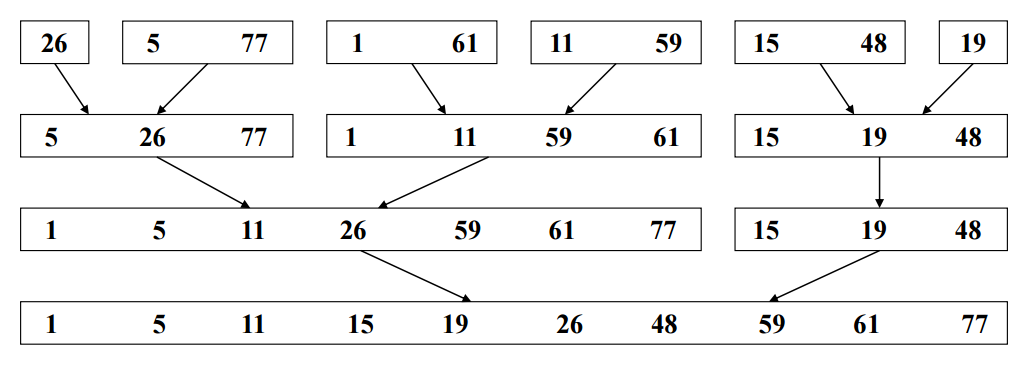
\includegraphics[width=.9\linewidth]{nmerge.PNG}
\caption*{7장 34페이지의 그림}
\end{figure}
일반적인 합병 정렬과 자연합병 정렬이 다른 것은, 일반적인 방법은 최초의 분할된 서브리스트의 길이가 1인 반면, 자연 합병 정렬은 오름차순이 보존된 단위로 시작한다는 것이다. 즉, 불필요한 정렬 과정을 뛰어 넘어 시간복잡도에서 이득을 얻어낸다.
자연 합병 정렬의 시간 복잡도는 $O(n\log n)$이다.(퀵 정렬과 매우 비슷하므로 설명 생략)\\
합병된 부분과 합병되지 않은 부분을 따로 저장해두어야 하므로, 저장공간이 많이 필요하다는 단점이 있다.
\pagebreak
\subsection{Heap sort : 히프 정렬}
히프정렬은 최대 히프를 이용해서 정렬하는 방법이다.
다음은 초기 최대 히프의 모습이다.
\begin{figure}[H]\centering
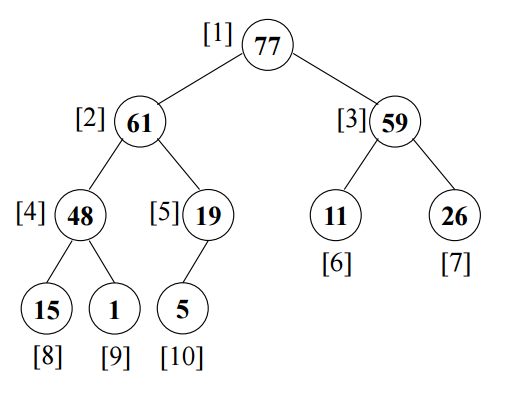
\includegraphics[width=.9\linewidth]{heap.PNG}
\caption*{7장 38페이지의 그림}
\end{figure}
최대 히프의 root에 위치한 레코드가 리스트의 최댓값이 된다는 성질을 이용하여, 최대 히프가 구성되고 나면, root값을 최대 히프의 마지막 index로 바꿔준다(그림에선 index=10의 5). 바꿔준 값으로 또 최대 히프를 만드는 작업을 수행한다. 각 단계에서 최대 히프를 만드는데, $O(\log n)$ 의 시간이 들고 n 단계를 거쳐 정렬이 완성되므로 최종 시간 복잡도로 $O(n\log n)$을 얻어낼 수 있다.
\subsection{정리}
각각의 정렬 방법은 데이터의 양상에 따라 매우 다른 시간복잡도를 보여 주었다. 이를 확인하기 위해 각 정렬에 대한 소스코드를 완성하고, 다른 양상으로 주어진 리스트를 정렬하여 걸리는 시간을 측정해보자.
\pagebreak

\section{소스코드}

\subsection{hw11.cpp}
\begin{lstlisting}
#include <iostream>
#include <fstream>
#include <ctime>
#include <stdlib.h>
#include <sys/time.h>
#include "sort.h"
using namespace std;
int main(int argc, char* argv[]) {
	int T = atoi(argv[1]); //` num of test case`
	cout << "T=" << T << endl;
	int N; //` 각 테스트케이스 별 레코드의 길이`
	int i; //` iterator`
	double result[4]; //` result 배열에 각 알고리즘 별로 실행시간을 저장하게 됩니다.`
	struct timeval start_t, end_t;
	double diff_t;
	if (argc < 3) {
		cerr << "wrong argument count" << endl;
		return 1;
	}
	cout << "--INS--|--QUICK--|--NATMG--|--HEAP--|" << endl;
	for (i = 2; i < T + 2; i++) {
		
		//`N개의 data를 읽어들인다.`
		fstream fin(argv[i]);
		fin>>N;
		int *data=new int[N];
		for(int j=0;j<N;j++) fin>>data[j];
		fin.close();
		
		//`Insertion sort`
		gettimeofday(&start_t, NULL);
		InsertionSort(data, N);
		gettimeofday(&end_t, NULL);
		diff_t = (double)(end_t.tv_sec-start_t.tv_sec)+
		((double)(end_t.tv_usec-start_t.tv_usec)/1000000);
		result[0] = diff_t;
		//`quicksort`
		gettimeofday(&start_t, NULL);
		QuickSort(data, N);
		gettimeofday(&end_t, NULL);
		diff_t = (double)(end_t.tv_sec-start_t.tv_sec)+
		((double)(end_t.tv_usec-start_t.tv_usec)/1000000);
		result[1] = diff_t;
		//`Natural Merge sort`
		gettimeofday(&start_t, NULL);
		NMergeSort(data, N);
		gettimeofday(&end_t, NULL);
		diff_t = (double)(end_t.tv_sec-start_t.tv_sec)+
		((double)(end_t.tv_usec-start_t.tv_usec)/1000000);
		result[2] = diff_t;
		//`Heapsort`
		gettimeofday(&start_t, NULL);
		HeapSort(data, N);
		gettimeofday(&end_t, NULL);
		diff_t = (double)(end_t.tv_sec-start_t.tv_sec)+
		((double)(end_t.tv_usec-start_t.tv_usec)/1000000);
		result[3] = diff_t;
		
		delete[] data;
		
		//`유효숫자를 5로 하여 출력`
		cout.precision(5);
		cout << fixed;
		for (int j = 0; j < 4; j++) {
			cout << result[j] << "|";
		}
		cout << "N=" << N << endl;
	}
}
\end{lstlisting}
\begin{figure}[H]
\caption*{설명은 주석으로 대체}
\end{figure}



\subsection{sort.h}
\begin{lstlisting}
#ifndef SORT_H
#define SORT_H
#include<iostream>
#include<iomanip>
using namespace std;
template <class T>
int verify(T* sorted, const int n){ //`정렬이 정상적으로 작동하는지 확인`
//`앞에 이상 없이 정렬된 data의 수를 return`
	int i=0;
	int* broken;
	int size=0;
	while(i<n-1){
		if(sorted[i]>sorted[i+1]) broken[size++]=i+1;
		i++;
	}
	if(size){
		cout<<"the number of broken parts : "<<size<<endl;
		for(int i=0;i<size;i++) cout<<i<<"st index : "<<sorted[broken[i]]<<endl;
		return broken[0]; //`최초로 정렬에 문제가 생긴 시점`
	}
	else return n;
}
//`테스트케이스를 보존하기 위해서 입력데이터를 복사한다.`
template <class T>
void Insert(const T& e, T* a, int i){
	a[0] = e;
	while(e < a[i]){ //`적절한 위치를 찾을 때까지`
		//`한 칸씩 앞으로 옮긴다`
		a[i + 1] = a[i];
		i--;
	}
	a[i + 1] = e;
}
template <class T>
void InsertionSort(T* data, const int n){
	T* a=new int[n+1];
	a[0]=0;
	copy(data,data+n,a+1); //`테스트케이스 보존 위함`
	for (int j = 2; j <= n; j++) {
		T temp = a[j]; //`오른쪽으로 계속 이동`
		Insert(temp, a, j - 1); //`시간복잡도 : O(j)`
	}
	//`int check=verify(a,n);
	//`cout<<setw(8)<<check;
	delete[] a; //`반드시 메모리 반납`
}
template <class T>
void QuickSort(T* a, const int left, const int right){
	//`iterative와 recursive 방식으로의 성능적 차이는 무시하도록 하자`
	if (left < right) { //`left==right 때까지`
		int i = left, j = right + 1, pivot = a[left]; //`리스트의 left를 pivot으로`
		do {
			do i++; while (a[i] < pivot); 
			do j--; while (a[j] > pivot); 
			if (i < j) swap(a[i], a[j]); //`회색영역으로 바꿔주는 작업`
		} while (i < j);
		swap(a[left], a[j]); 
		QuickSort(a, left, j - 1);
		QuickSort(a, j + 1, right); //`왼쪽리스트 정렬 끝나면 오른쪽 리스트 정렬 시작`
	}
}
template <class T>
void QuickSort(T* data, const int n){
	//`입력 리스트 보존과 정렬의 완성을 확인하기 위해 driver을 따로 정의`
	T* a=new int[n];
	copy(data,data+n,a);
	QuickSort(a,0,n-1);
	//`int check=verify(a,n);
	//`cout<<setw(8)<<check;
	delete[] a;
}
template <class T>
void Merge(T* initList, T* mergedList, const int l, const int m, const int n){ 
	//`l부터 m까지, m+1부터 n까지 정렬된 상태`
	int i1, iResult, i2; 
	//`2장의 polynomial add와 방식이 같다`
	for (i1 = l, iResult = l, i2 = m + 1; 
		i1 <= m && i2 <= n; 
		iResult++){
		//`왼쪽과 오른쪽 중에서 작은 값을 현재 위치에`
		if (initList[i1] <= initList[i2]) {
			mergedList[iResult] = initList[i1];
			i1++;
		}
		else {
			mergedList[iResult] = initList[i2];
			i2++;
		}
	}
	//`i1<=m||i2<=n 의 상황`
	copy(initList + i1, initList + m + 1, mergedList + iResult);
	copy(initList + i2, initList + n + 1, mergedList + iResult);
}
//`자연 합병 정렬`
template <class T>
void NMergePass(T* initList, T* resultList, const int n, int* length, int size){
	Merge(initList, resultList, 0, length[0], length[1]);
	//`size만큼 서브리스트를 합쳐준다. (잘못된 위치를 읽지 않도록 주의!!)`
	for (int i=1;i<size-2;i+=2) 
		Merge(initList, resultList, length[i]+1, length[i+1], length[i+2]);
}
template <class T>
void NMergeSort(T* data, const int n){ 
	T* a=new int[n];
	copy(data,data+n,a);
	T* tempList = new T[n + 1];
	int length[n]; //`서브리스트들의 길이를 담는다`
	fill(length,length+n+1,0);
	int pos=0;
	int size; //`length의 크기`
	for(size=0;pos<n;size++){ //`최초 서브리스트 생성`
		while(a[pos]<=a[pos+1]&&pos<n-1) pos++; //`오름차순 보존된 곳까지`
		length[size]=pos;
		pos++;
	}
	while(size>1){ //`서브리스트가 1개일 때 : 한개로 합쳐질 때까지 `
		NMergePass(a,tempList,n,length,size);
		//`length 갱신`
		for(int i=0;i<size/2;i++) length[i]=length[2*i+1]; //`합쳐진 길이는 오른쪽 리스트의 끝`
		//`이전 단계의 서브리스트 수가 짝수였을 때 마지막 위치보존`		
		if(size%2) length[size/2]=length[size-1];
		size=(size+1)/2;
		NMergePass(tempList,a,n,length,size);
	}
	//`int check=verify(a,n);
	//`cout<<setw(8)<<check;
	delete[] tempList;
	delete[] a;
}
template <class T>
void Adjust(T* a, const int root, const int n){ //`n : 남은 레코드 수`
	//`최대 히프로 만드는 작업`
	T e = a[root];
	int j; 
	for (j = 2 * root; j <= n; j *= 2) { //`j*2 : j의 parent`
		if (j < n && a[j] < a[j + 1]) j++; //`siblling의 우위 결정 `
		if (e >= a[j]) break; //`적절한 위치`
		a[j / 2] = a[j]; 
	}
	a[j / 2] = e; 
}
template <class T>
void HeapSort(T* data, const int n){
	T* a=new int[n+1];
	a[0]=0;
	copy(data,data+n,a+1);
	for (int i = n / 2; i >= 1; i--) Adjust(a, i, n); //`최초 최대 히프 구성`
	for (int i = n - 1; i >= 1; i--) {
		//`최대히프 구성 후, 마지막 위치를 root와 swap 후 다시 최대히프 구성`
		swap(a[1], a[i + 1]);
		Adjust(a, 1, i); 
	}
	//`int check=verify(a,n);
	//`cout<<setw(8)<<check;
	delete[] a;
}
#endif

\end{lstlisting}
\begin{figure}[H]
\caption*{설명은 주석으로 대체}
\end{figure}

\pagebreak
\section{결과 해석 및 분석 : testcases 실행}
위의 소스코드를 바탕으로 다양한 분포의 리스트를 입력하고자 한다.
분포는 다음과 같다.
\begin{quote}\centering
    random\;\;\;\;decreasing\;\;\;\;partially sorted\;\;\;\;sorted
\end{quote}
각각의 분포 당 12개의 테스트케이스를 입력받고, 각각의 테스트케이스에 포함된 레코드의 수는 다음과 같다.
\begin{quote}\centering
    50, 100, 200, 300, 500, 1000, 3000, 5000, 10000, 30000, 50000, 100000
\end{quote}
\textit{그래프가 직관적으로 와닿지 않을 수 있으니 왼쪽의 시간 값들로 비교한다.}

\arrayrulecolor{black}
\subsection{random 분포}
\begin{figure}[H]
\begin{subfigure}[ht]{.3\linewidth}\centering
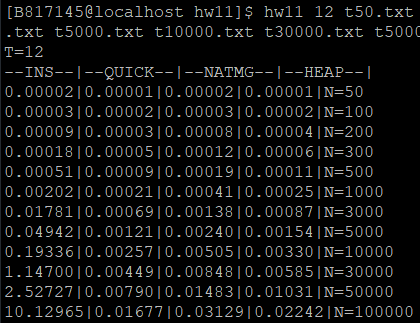
\includegraphics[width=.9\linewidth]{random2.PNG}
\subcaption*{테스트케이스별 시간값}
\end{subfigure}
\begin{subfigure}[ht]{.7\linewidth}\centering
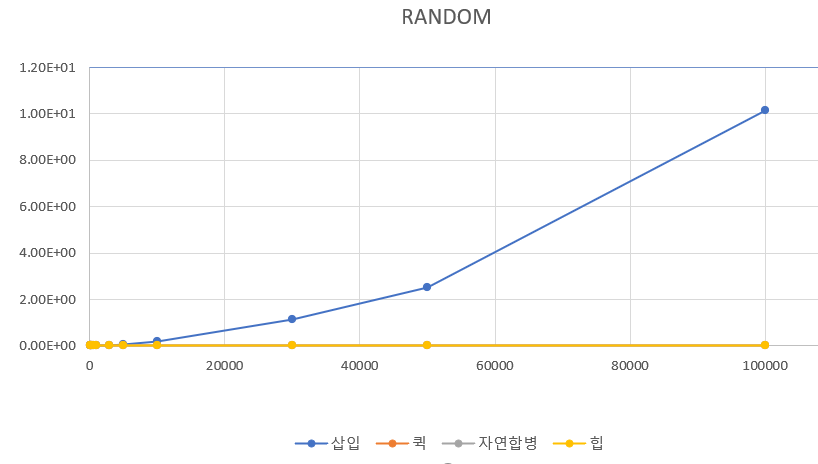
\includegraphics[width=.9\linewidth]{random.PNG}
\subcaption*{x축 : 레코드 수 y축 : 걸린 시간}
\end{subfigure}
\end{figure}
\begin{table}[H]
\centering
\begin{tabular}{|m{15cm}|}
\hline
분포가 무작위일때, quick sort의 성능이 가장 좋은 것을 확인 할 수가 있다.\\
N=50000 과 N=100000을 보면, \\
insertion sort에서, 레코드의 수가 2배이므로 약 4배의 시간이 걸리는 것을 확인할 수 있다.\\
그 외의 정렬에서, 2배의 시간이 걸리는 것을 확인할 수 있다.($\frac{100000\log 100000}{50000\log 50000}\simeq 2$) \\
\hline
\end{tabular}
\end{table}

\subsection{decreasing 분포}
\begin{figure}[H]
\begin{subfigure}[ht]{.3\linewidth}\centering
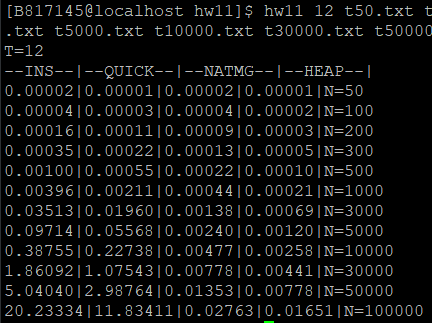
\includegraphics[width=.9\linewidth]{decreasing2.PNG}
\subcaption*{테스트케이스별 시간값}
\end{subfigure}
\begin{subfigure}[ht]{.7\linewidth}\centering
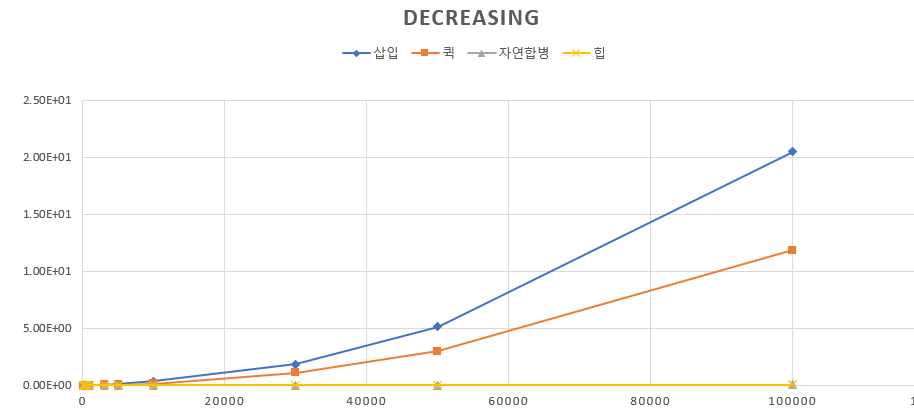
\includegraphics[width=.9\linewidth]{decreasing.PNG}
\subcaption*{x축 : 레코드 수 y축 : 걸린 시간}
\end{subfigure}
\end{figure}
\begin{table}[H]
\centering
\begin{tabular}{|m{15cm}|}
\hline
quicksort의 시간복잡도가 $O(n^2)$임을 확인한다.\\
N=50000 과 N=100000을 보면, isertion sort과 마찬가지로 약 4배의 시간이 걸린다.\\
나머지는 테스트케이스별 걸리는 시간의 배수가 random과 비슷하다.\\
\hline
\end{tabular}
\end{table}

\subsection{partially sorted 분포}
\begin{figure}[H]
\begin{subfigure}[ht]{.3\linewidth}\centering
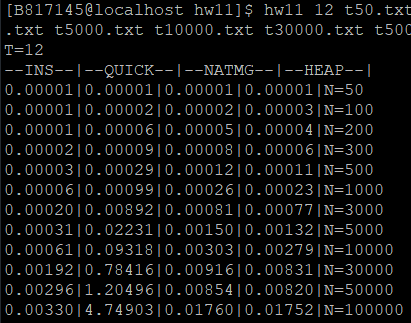
\includegraphics[width=.9\linewidth]{partially2.PNG}
\subcaption*{테스트케이스별 시간값}
\end{subfigure}
\begin{subfigure}[ht]{.7\linewidth}\centering
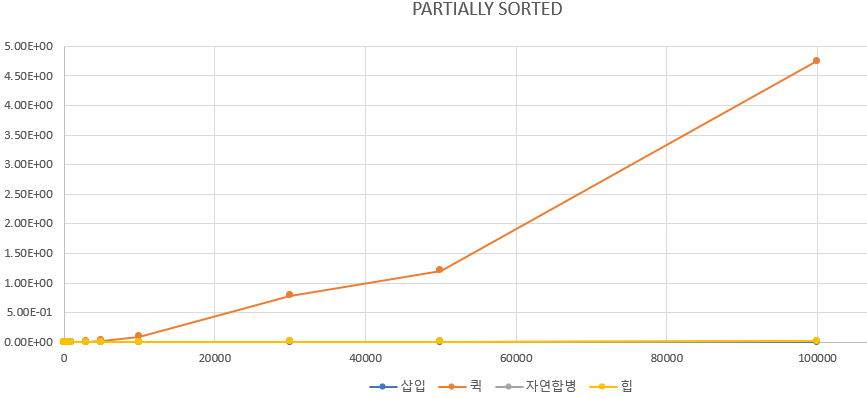
\includegraphics[width=.9\linewidth]{partially.PNG}
\subcaption*{x축 : 레코드 수 y축 : 걸린 시간}
\end{subfigure}
\end{figure}
\begin{table}[H]
\centering
\begin{tabular}{|m{15cm}|}
\hline
insertion sort의 시간이 다른 분포에 비해 눈에 띠게 줄어든 것을 확인할 수 있다.\\
heapsort와 natural mergesort의 시간이 거의 비슷함을 확인할 수 있다.\\
\hline
\end{tabular}
\end{table}


\subsection{sorted 분포}
\begin{figure}[H]
\begin{subfigure}[ht]{.3\linewidth}\centering
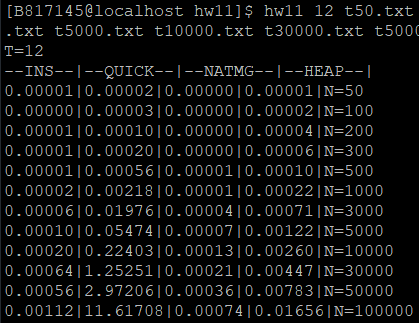
\includegraphics[width=.9\linewidth]{sorted2.PNG}
\subcaption*{테스트케이스별 시간값}
\end{subfigure}
\begin{subfigure}[ht]{.7\linewidth}\centering
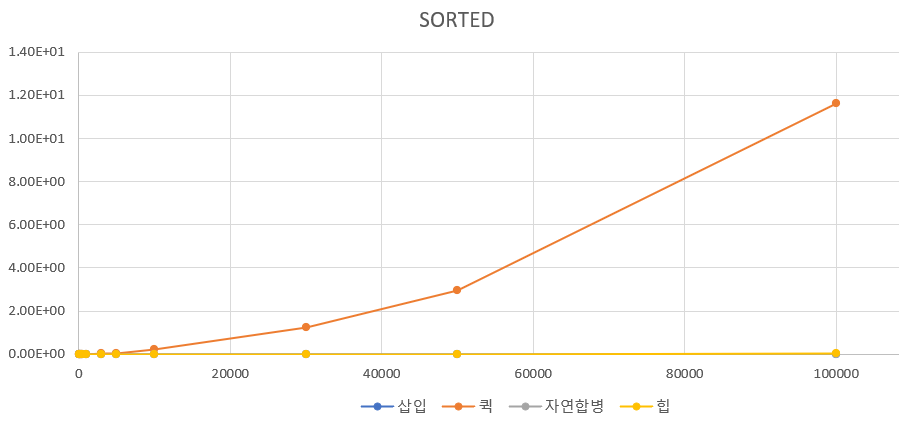
\includegraphics[width=.9\linewidth]{sorted.PNG}
\subcaption*{x축 : 레코드 수 y축 : 걸린 시간}
\end{subfigure}
\end{figure}
\begin{table}[H]
\centering
\begin{tabular}{|m{15cm}|}
\hline
quick sort가 걸리는 시간이 decreasing 분포일 때와 비슷하다.\\
insertion sort의 성능이 매우 향상되었음을 확인한다.\\
N=300 이후로 시간이 선형적으로 변하는 것을 확인할 수 있다.\\
(사실상 n개의 레코드를 순회하는 시간이다.)\\
이는 natural merge sort에서도 확인할 수 있다.\\
\hline
\end{tabular}
\end{table}

\subsection{정리}
서로 다른 분포에서, 각각의 정렬이 가진 특징들을 확인할 수 있었다. 무작위 분포에서 우수한 quick sort와 분포에 상관없이 일정한 성능의 heapsort, 부분 정렬된 분포에서 성능이 향상되는insertion sort을 확인하였다. 또한, 각 분포에서 natural merge sort와 heapsort이 각 시간별로 비례함도 확인했다.\\

\end{document}